\section{Cortes Clique}

\bigskip
\subsection{Formulaci\'on}
\label{formulacion}

Lo cortes clique como el nombre lo indica requieren alg\'un grafo subyacente del cual se puedan inferir cortes.
Ante\'es de explicar los cortes, se comenta el grafo de nuestro problema.

Las instancias a resolver fueron restringidas a instancias con todas las variables binarias.
Existen grafos que sirven para representar este tipo de problemas y son los \emph{grafos de conflictos}.
Lo que dice el grafo de conflicto es si existen combinaciones de pares de nodos que no pueden ocurrir, es decir,
dadas las restricciones de nuestro problema puede existir variables $x_2$ y $x_3$ tal que que si las dos estan en 1,
el conjunto de restricciones se vuelve infactible(como en la desigualdad ~\ref{eq1}). De la misma manera puede ocurrir que $x_2$ este en 1, y $x_1$ esta en 0 y que tambi\'en
as\'i el conjunto de resticciones sea infactible (como en la desigualdad ~\ref{eq2}).

\begin{equation} \label{eq1}
-3 x_1 + 3 x_2 + 5 x_3 \leq 3
\end{equation}
\begin{equation} \label{eq2}
4 x_1 - 1 x_2 + 3 x_3 \geq 3
\end{equation}

Por lo tanto, existen combinaciones de pares de nodos que no pueden ocurrir en una soluci\'on del problema, cada combinaci\'on que no pueda ocurrir
es un eje en nuestro grafo de conflictos. Para representar este grafo, se tiene un conjunto $\mathcal{V}$ dos nodos por cada variable, $x_i$
representando la variable $x_i$ en 1, y $\tilde{x}_i$ para la variable $x_i$ en 0. Por lo tanto, el conjunto $\mathcal{E}$ de ejes son los pares de 
nodos que no pueden ocurrir en nuestro problema, entre ellos, los que conectan a $x_i$ con $\tilde{x}_i$ como muestra la figura ~\ref{fig1}.


\begin{figure}[H]
\begin{center}
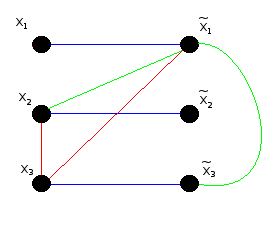
\includegraphics{grafoconflicto}
\end{center}
\caption{Grafo de conflictos del las restricciones anteriores}
\label{fig1}
\end{figure}

Una vez que se tiene armado el grafo, se puede ver que las soluciones factibles, son en realidad \emph{conjuntos independientes} en nuestro grafo
(ie: no existen dos nodos conectados con un eje, porque estan conectas las que hacen problema infactible). Por lo tanto cada eje representa
tambi\'en una restricci\'on en el problema dependiendo la combinaci\'on variables.

\begin{itemize}
\item Si los nodos $x_i$ y $x_j$ son vecinos se tiene una restricci\'on del estilo $x_i +x_j \leq 1$
\item Si los nodos $x_i$ y $\tilde{x}_j$ son vecinos se tiene una restricci\'on del estilo $x_i + 1-x_j \leq 1$
\item Si los nodos $\tilde{x}_i$ y $x_j$ son vecinos se tiene una restricci\'on del estilo $1-x_i +x_j \leq 1$
\item Si los nodos $\tilde{x}_i$ y $\tilde{x}_j$ son vecinos se tiene una restricci\'on del estilo $1-x_i + 1-x_j \leq 1$
\end{itemize}

Una idea ingenua podria insertar todos estas restricciones a nuestra formulaci\'on del problema lineal, reduciendo as\'i la posibilidad de que soluciones no factibles.
Pero al aumentar la cantidad de resticciones considerablemente, se tarda m\'as en resolver el problema por el m\'etodo simplex. Por lo que se va
a insertar las restricciones a medida que resulten convenientes.

Cuando resulta conveniente? Si en la relajaci\'on lineal se viola alguna restricci\'on, va a ser conveniente cortar soluciones de ese tipo.
Como la soluci\'on ser\'a un conjunto independiente en el grafo de conflictos, entonces, todas las cliques en nuestro grafo tienen a lo sumo
un nodo como parte de la soluci\'on. Entonces si al encontrar la relajaci\'on lineal se encuenta una clique que viole esta condici\'on, entonces
la resticci\'on de que en la clique debe haber a lo sumo un nodo elegido sera \'util para cortar soluciones.

\begin{equation} \label{eq3}
\sum\limits_{i \in \mathcal{K}} x_i \leq 1
\end{equation}

\bigskip
\subsection{Construcci\'on del grafo}

Lo primero a realizar es construir el grafo de conflictos que se menciona en la secci\'on ~\ref{formulacion}.
Si la instancia del problema lo permite, es posible recorrer todas las posibilidades por fuerza bruta. Es decir, para cada par de variables y para cada 
combinaci\'on de variable en 1 y variable en 0, se evalua si el conjunto de restricciones es infactible.

Para ver si el conjunto de restricciones es factible dado que dos variables tienen un valor fijo, se busca
todas las restricciones que contengan a estas dos variables y ver si existe una valuaci\'on tal que sea factible. Esto se puede hacer de manera
golosa, ya que la resticciones que son por menor o igual, basta poner en 1 todas las variables con coeficiente negativo, y en 0 todas las variables que tengan coeficiente positivo. Si usando
esta valuaci\'on la restricci\'on resulta infactible se puede probar que el conjunto de restricciones es infactible para esta combinaci\'on de nodos. De manera analoga para las restricciones
 por mayor o igual, se intenta que las variables que tengan coeficiente positivo esten en 1, y las dem\'as en 0 (recordando que hay 2 nodos cuyo valor es fijo).

Para los casos donde no sea posible realizar fuerza bruta (ya sea porque hay demasiados ejes en el grafo de conflictos, o porque tarda demasiado),
es posible quedarse  con un conjunto al azar de variables, y probar sobre estas si existen ejes.

\bigskip
\subsection{Algoritmo de separaci\'on}

Una vez que tenemos la relajaci\'on lineal, lo que buscamos es la clique de mayor peso en el grafo de conflictos. Dicho problema es {\bf NP-completo},
por lo que se realiza un heurisitica para encontrar algunas cliques candidatas ya que no es posible resolverlo de forma exacta. 

Teniendo la clique de mayor peso, es puede determinar si esta clique esta violando las restricciones si la suma de sus variables es mayor a 1. En caso 
de que as\'i sea, se inserta la restricci\'on clique (desigualdad ~\ref{eq3}) al LP.

\newpage 

\begin{algorithmic}
\label{algo3}
\Function{GenerarClique}{k,s} \Comment{k es una clique,s es el primer nodo no usado}
  \For{$i \gets s \textrm{ to } n$}
    \If{$i \textrm{ tiene eje con todos en } k$}
     \State $GenerarClique(k+i,i+1)$ \Comment{Agregamos el nodo i a la clique}
    \EndIf
  \EndFor
  \If{Ning\'un nodo pudo entrar a la clique}
     \If{Suma de relajaciones de k mayor a 1}$MeterRestriccion(k)$
     \EndIf
  \EndIf
\EndFunction
\end{algorithmic}
\bigskip

La heurisitica presentada consiste en encontrar cliques maximales que sean candidatas a cortar el grafo. Primero se ordena a los
nodos por su valor en la relajaci\'on lineal. Luego se intenta insertar cada nodo en la clique como indica el algoritmo GenerarClique. De esta manera
el resultado es una clique maximal, y se puede evaluar si viola el conjunto de resticciones.

Como la cantidad de cliques en un grafo puede ser muy grande, la heurisitica debe dejar de buscar cliques en alg\'un momento, por lo que se puede
fijar en algun par\'ametro cuantas cliques se decide explorar.
Una desventaja de esto es que a medida que se acerca a la soluci\'on, puede pasar que el orden de los nodos no varie mucho, resultando en explorar siempre las misma cliques.







